% A.B.B. Dynamic vs. A.B.B. Greedy 
% Written by Edisson López 
% Contact: ediloaz@gmail.com 
% Cartago, Costa Rica 
  
% For the course: 
% 	Operations Research (of Costa Rica Institute of Technology) 
% 	Teacher: Dr. Jose Francisco Torres 
 
% HEADER { 
\documentclass[a4paper,twocolumn,10pt]{article} 
\usepackage{tikz} 
\usepackage{pgfplots} 
\pgfplotsset{compat=1.10} 
\usetikzlibrary{shapes.geometric,arrows,fit,matrix,positioning} 
\tikzset 
{ 
    treenode/.style = {circle, draw=black, align=center, minimum size=1cm} 
} 
\usepackage{lmodern} 
\usepackage{float} 
\usepackage[T1]{fontenc} 
%\usepackage[spanish]{babel} 
\usepackage[utf8]{inputenc} 
\usepackage[left=0.7cm, top=1.5cm, right=0.7cm, bottom=2cm]{geometry} 
\newcommand\tab[1][1cm]{\hspace*{#1}} 
\newcommand\minitab[1][0.5cm]{\hspace*{#1}} 
\title{A.B.B. Dynamic vs. A.B.B. Greedy} 
\author{Edisson López Díaz} 
\date{\today}  
% } HEADER 
% DOCUMENT { 
\begin{document} 
\maketitle 

\section{"Example" mode} 
\subsection*{Initial problem} 
\textbf{Six keys} random were generated, with these we proceed to find the optimal solution with the Greedy algorithm and the dynamic programming algorithm.\\ 
Keys generated: \\ 
\tab Key \minitab Weight \minitab Probability \\ 
\tab KeyA \minitab  743 \tab 0.308043 \\ 
 \tab KeyB \minitab  124 \tab 0.051410 \\ 
 \tab KeyC \minitab  837 \tab 0.347015 \\ 
 \tab KeyD \minitab  149 \tab 0.061774 \\ 
 \tab KeyE \minitab  512 \tab 0.212272 \\ 
 \tab KeyF \minitab  47 \tab 0.019486 \\ 
 
Forced sum of the probability of the keys: 1.0 \\ 
\subsection{Greedy Aagorithm} 
From the previous keys we create an equivalent to the R table used in the dynamic programming algorithm. Choosing each time the key of maximum probability to be the root of the tree, separating the rest of the keys into two groups: the minor ones that the selected root and the majors that this root. This recursively. 
\begin{center} 
\textbf{Tabla R} \\ 
\begin{tabular}{|c|c|c|c|c|c|c|c|}
\hline \textbf{•} & \textbf{0}& \textbf{1}& \textbf{2}& \textbf{3}& \textbf{4}& \textbf{5}& \textbf{6}\\ \hline 
\textbf{1} & 0 & 1 & \textbf{1} &  &  &  & \textbf{3} \\ 
\hline 
\textbf{2} &  & 0 & 2 &  &  &  &  \\ 
\hline 
\textbf{3} &  &  & 0 & 3 &  &  &  \\ 
\hline 
\textbf{4} &  &  &  & 0 & 4 &  & \textbf{5} \\ 
\hline 
\textbf{5} &  &  &  &  & 0 & 5 &  \\ 
\hline 
\textbf{6} &  &  &  &  &  & 0 & 6 \\ 
\hline 
\textbf{7} &  &  &  &  &  &  & 0 \\ 
\hline 
\end{tabular} 
\end{center} 
\begin{figure}[H] 
\begin{center} 
Optimal tree created from table R \\ 
{ 
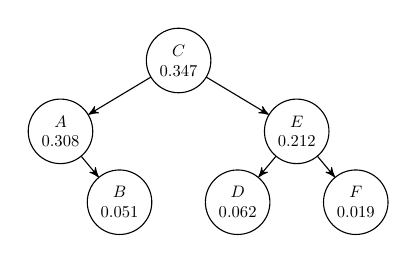
\begin{tikzpicture}[->,>=stealth',level/.style={sibling distance = 5cm/#1, level distance = 1.5cm},scale=0.6, transform shape] 
\node [treenode] {$C$   \\ 0.347}  child { 
node [treenode] {$A$   \\ 0.308}  child[missing] child { node [treenode] {$B$   \\ 0.051}  } 
} 
child { node [treenode] {$E$   \\ 0.212}  child { 
node [treenode] {$D$   \\ 0.062}  } 
child { node [treenode] {$F$   \\ 0.019}  } 
} 
; 
\end{tikzpicture}  
}  
\end{center} 
\end{figure} 

\textbf{Computing time: } 39 microseconds 
\subsection{Dynamic algorithm} 

From the previous keys the following table is created: \\ 
\begin{center} 
\textbf{Tabla A} \\ 
\begin{tabular}{|c|c|c|c|c|c|c|c|}
\hline \textbf{•} & \textbf{0}& \textbf{1}& \textbf{2}& \textbf{3}& \textbf{4}& \textbf{5}& \textbf{6}\\ \hline 
\textbf{1} & 0.000 & 0.308 & 0.000 & 0.000 & 0.000 & 0.000 & 0.000 \\ 
\hline 
\textbf{2} &  & 0.000 & 0.051 & 0.000 & 0.000 & 0.000 & 0.000 \\ 
\hline 
\textbf{3} &  &  & 0.000 & 0.347 & 0.000 & 0.000 & 0.000 \\ 
\hline 
\textbf{4} &  &  &  & 0.000 & 0.062 & 0.000 & 0.000 \\ 
\hline 
\textbf{5} &  &  &  &  & 0.000 & 0.212 & 0.000 \\ 
\hline 
\textbf{6} &  &  &  &  &  & 0.000 & 0.019 \\ 
\hline 
\textbf{7} &  &  &  &  &  &  & 0.000 \\ 
\hline 
\end{tabular} 
\end{center} 
Now proceed to complete Tabla A and R, calculating and choosing the value of each cell of said tables. \\ 
 
Calculation for the cell \textbf{[5][6]}: \\ 
\tab A[5][4] + A[6][6] = 0.000 + 0.019 = 0.019 *min*\\ 
\tab A[5][5] + A[7][6] = 0.212 + 0.000 = 0.212\\ 
\minitab K winner: 5 \\ 
\minitab Selected: [5][4] + [6][6] + Ks = \textbf{0.251244} \\ 
 
Calculation for the cell \textbf{[4][5]}: \\ 
\tab A[4][3] + A[5][5] = 0.000 + 0.212 = 0.212 *min*\\ 
\tab A[4][4] + A[6][5] = 0.062 + 0.000 = 0.062 *min*\\ 
\minitab K winner: 5 \\ 
\minitab Selected: [4][4] + [6][5] + Ks = \textbf{0.335821} \\ 
 
Calculation for the cell \textbf{[3][4]}: \\ 
\tab A[3][2] + A[4][4] = 0.000 + 0.062 = 0.062 *min*\\ 
\tab A[3][3] + A[5][4] = 0.347 + 0.000 = 0.347\\ 
\minitab K winner: 3 \\ 
\minitab Selected: [3][2] + [4][4] + Ks = \textbf{0.470564} \\ 
 
Calculation for the cell \textbf{[2][3]}: \\ 
\tab A[2][1] + A[3][3] = 0.000 + 0.347 = 0.347 *min*\\ 
\tab A[2][2] + A[4][3] = 0.051 + 0.000 = 0.051 *min*\\ 
\minitab K winner: 3 \\ 
\minitab Selected: [2][2] + [4][3] + Ks = \textbf{0.449834} \\ 
 
Calculation for the cell \textbf{[1][2]}: \\ 
\tab A[1][0] + A[2][2] = 0.000 + 0.051 = 0.051 *min*\\ 
\tab A[1][1] + A[3][2] = 0.308 + 0.000 = 0.308\\ 
\minitab K winner: 1 \\ 
\minitab Selected: [1][0] + [2][2] + Ks = \textbf{0.410862} \\ 
 
Calculation for the cell \textbf{[4][6]}: \\ 
\tab A[4][3] + A[5][6] = 0.000 + 0.251 = 0.251 *min*\\ 
\tab A[4][4] + A[6][6] = 0.062 + 0.019 = 0.081 *min*\\ 
\tab A[4][5] + A[7][6] = 0.336 + 0.000 = 0.336\\ 
\minitab K winner: 5 \\ 
\minitab Selected: [4][4] + [6][6] + Ks = \textbf{0.374793} \\ 
 
Calculation for the cell \textbf{[3][5]}: \\ 
\tab A[3][2] + A[4][5] = 0.000 + 0.336 = 0.336 *min*\\ 
\tab A[3][3] + A[5][5] = 0.347 + 0.212 = 0.559\\ 
\tab A[3][4] + A[6][5] = 0.471 + 0.000 = 0.471\\ 
\minitab K winner: 3 \\ 
\minitab Selected: [3][2] + [4][5] + Ks = \textbf{0.956882} \\ 
 
Calculation for the cell \textbf{[2][4]}: \\ 
\tab A[2][1] + A[3][4] = 0.000 + 0.471 = 0.471 *min*\\ 
\tab A[2][2] + A[4][4] = 0.051 + 0.062 = 0.113 *min*\\ 
\tab A[2][3] + A[5][4] = 0.450 + 0.000 = 0.450\\ 
\minitab K winner: 3 \\ 
\minitab Selected: [2][2] + [4][4] + Ks = \textbf{0.573383} \\ 
 
Calculation for the cell \textbf{[1][3]}: \\ 
\tab A[1][0] + A[2][3] = 0.000 + 0.450 = 0.450 *min*\\ 
\tab A[1][1] + A[3][3] = 0.308 + 0.347 = 0.655\\ 
\tab A[1][2] + A[4][3] = 0.411 + 0.000 = 0.411 *min*\\ 
\minitab K winner: 3 \\ 
\minitab Selected: [1][2] + [4][3] + Ks = \textbf{1.117330} \\ 
 
Calculation for the cell \textbf{[3][6]}: \\ 
\tab A[3][2] + A[4][6] = 0.000 + 0.375 = 0.375 *min*\\ 
\tab A[3][3] + A[5][6] = 0.347 + 0.251 = 0.598\\ 
\tab A[3][4] + A[6][6] = 0.471 + 0.019 = 0.490\\ 
\tab A[3][5] + A[7][6] = 0.957 + 0.000 = 0.957\\ 
\minitab K winner: 3 \\ 
\minitab Selected: [3][2] + [4][6] + Ks = \textbf{1.015340} \\ 
 
Calculation for the cell \textbf{[2][5]}: \\ 
\tab A[2][1] + A[3][5] = 0.000 + 0.957 = 0.957 *min*\\ 
\tab A[2][2] + A[4][5] = 0.051 + 0.336 = 0.387 *min*\\ 
\tab A[2][3] + A[5][5] = 0.450 + 0.212 = 0.662\\ 
\tab A[2][4] + A[6][5] = 0.573 + 0.000 = 0.573\\ 
\minitab K winner: 3 \\ 
\minitab Selected: [2][2] + [4][5] + Ks = \textbf{1.059702} \\ 
 
Calculation for the cell \textbf{[1][4]}: \\ 
\tab A[1][0] + A[2][4] = 0.000 + 0.573 = 0.573 *min*\\ 
\tab A[1][1] + A[3][4] = 0.308 + 0.471 = 0.779\\ 
\tab A[1][2] + A[4][4] = 0.411 + 0.062 = 0.473 *min*\\ 
\tab A[1][3] + A[5][4] = 1.117 + 0.000 = 1.117\\ 
\minitab K winner: 3 \\ 
\minitab Selected: [1][2] + [4][4] + Ks = \textbf{1.240879} \\ 
 
Calculation for the cell \textbf{[2][6]}: \\ 
\tab A[2][1] + A[3][6] = 0.000 + 1.015 = 1.015 *min*\\ 
\tab A[2][2] + A[4][6] = 0.051 + 0.375 = 0.426 *min*\\ 
\tab A[2][3] + A[5][6] = 0.450 + 0.251 = 0.701\\ 
\tab A[2][4] + A[6][6] = 0.573 + 0.019 = 0.593\\ 
\tab A[2][5] + A[7][6] = 1.060 + 0.000 = 1.060\\ 
\minitab K winner: 3 \\ 
\minitab Selected: [2][2] + [4][6] + Ks = \textbf{1.118159} \\ 
 
Calculation for the cell \textbf{[1][5]}: \\ 
\tab A[1][0] + A[2][5] = 0.000 + 1.060 = 1.060 *min*\\ 
\tab A[1][1] + A[3][5] = 0.308 + 0.957 = 1.265\\ 
\tab A[1][2] + A[4][5] = 0.411 + 0.336 = 0.747 *min*\\ 
\tab A[1][3] + A[5][5] = 1.117 + 0.212 = 1.330\\ 
\tab A[1][4] + A[6][5] = 1.241 + 0.000 = 1.241\\ 
\minitab K winner: 3 \\ 
\minitab Selected: [1][2] + [4][5] + Ks = \textbf{1.727197} \\ 
 
Calculation for the cell \textbf{[1][6]}: \\ 
\tab A[1][0] + A[2][6] = 0.000 + 1.118 = 1.118 *min*\\ 
\tab A[1][1] + A[3][6] = 0.308 + 1.015 = 1.323\\ 
\tab A[1][2] + A[4][6] = 0.411 + 0.375 = 0.786 *min*\\ 
\tab A[1][3] + A[5][6] = 1.117 + 0.251 = 1.369\\ 
\tab A[1][4] + A[6][6] = 1.241 + 0.019 = 1.260\\ 
\tab A[1][5] + A[7][6] = 1.727 + 0.000 = 1.727\\ 
\minitab K winner: 3 \\ 
\minitab Selected: [1][2] + [4][6] + Ks = \textbf{1.785655} \\ 

 After the calculation process, the following tables are obtained: 
\begin{center} 
\textbf{Tabla A} \\ 
\begin{tabular}{|c|c|c|c|c|c|c|c|}
\hline \textbf{•} & \textbf{0}& \textbf{1}& \textbf{2}& \textbf{3}& \textbf{4}& \textbf{5}& \textbf{6}\\ \hline 
\textbf{1} & 0.000 & 0.308 & 0.411 & 1.117 & 1.241 & 1.727 & 1.786 \\ 
\hline 
\textbf{2} &  & 0.000 & 0.051 & 0.450 & 0.573 & 1.060 & 1.118 \\ 
\hline 
\textbf{3} &  &  & 0.000 & 0.347 & 0.471 & 0.957 & 1.015 \\ 
\hline 
\textbf{4} &  &  &  & 0.000 & 0.062 & 0.336 & 0.375 \\ 
\hline 
\textbf{5} &  &  &  &  & 0.000 & 0.212 & 0.251 \\ 
\hline 
\textbf{6} &  &  &  &  &  & 0.000 & 0.019 \\ 
\hline 
\textbf{7} &  &  &  &  &  &  & 0.000 \\ 
\hline 
\end{tabular} 
\end{center} 
\begin{center} 
\textbf{Tabla R} \\ 
\begin{tabular}{|c|c|c|c|c|c|c|c|}
\hline \textbf{•} & \textbf{0}& \textbf{1}& \textbf{2}& \textbf{3}& \textbf{4}& \textbf{5}& \textbf{6}\\ \hline 
\textbf{1} & 0 & 1 & 1 & 3 & 3 & 3 & 3 \\ 
\hline 
\textbf{2} &  & 0 & 2 & 3 & 3 & 3 & 3 \\ 
\hline 
\textbf{3} &  &  & 0 & 3 & 3 & 3 & 3 \\ 
\hline 
\textbf{4} &  &  &  & 0 & 4 & 5 & 5 \\ 
\hline 
\textbf{5} &  &  &  &  & 0 & 5 & 5 \\ 
\hline 
\textbf{6} &  &  &  &  &  & 0 & 6 \\ 
\hline 
\textbf{7} &  &  &  &  &  &  & 0 \\ 
\hline 
\end{tabular} 
\end{center} 
\begin{figure}[H] 
\begin{center} 
Optimal tree created from table R \\ 
{ 
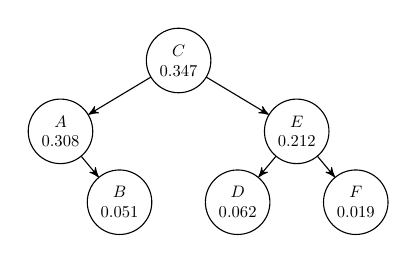
\begin{tikzpicture}[->,>=stealth',level/.style={sibling distance = 5cm/#1, level distance = 1.5cm},scale=0.6, transform shape] 
\node [treenode] {$C$   \\ 0.347}  child { 
node [treenode] {$A$   \\ 0.308}  child[missing] child { node [treenode] {$B$   \\ 0.051}  } 
} 
child { node [treenode] {$E$   \\ 0.212}  child { 
node [treenode] {$D$   \\ 0.062}  } 
child { node [treenode] {$F$   \\ 0.019}  } 
} 
; 
\end{tikzpicture}  
}  
\end{center} 
\end{figure} 

\textbf{Computing time: } 504 microseconds 

\subsection*{Conclusions} 
\begin{itemize}

\item The two generated trees (greedy and dynamic programming) share the same topology, so both found the optimal solution. 
\item The computing time of the dynamic algorithm was 12 was less fast than the Greedy algorithm. 
\item With six keys the Greedy algorithm approximately the 32\% of the time finds the optimal solution. 
\end{itemize}
\end{document}
% } DOCUMENT 
% Last line of the document